\documentclass{article}
\usepackage[spanish]{babel}
\usepackage[a4paper,top=2cm,bottom=2cm,left=2cm,right=2cm,marginparwidth=1.5cm]{geometry}
\usepackage[colorlinks=true, allcolors=blue]{hyperref}
\usepackage{tabularx} % para autoajustar las tablas según contenido del texto
\usepackage{changepage} % para ajuste de márgenes
\usepackage{graphicx}
\usepackage{subcaption}
\usepackage{placeins} % Para fijar texto entre gráficos

\title{\textbf{Análisis de los Ingresos Principales en Chile: Una Perspectiva Demográfica, Regional y Comparativa con el Sueldo Mínimo}}
\author{Camilo Riquelme Horta}
\date{28.06.2024}

\begin{document}
	
	\begin{minipage}{0.5\textwidth}
		\begin{flushleft}
			Universidad Mayor \\Facultad de Ciencias, Ingeniería y Tecnología \\Carrera de Data Science
		\end{flushleft}
	\end{minipage}
	\begin{minipage}{0.5\textwidth}
		\begin{flushright}
			Taller de Ciencia de Datos I \\Profesor: Felipe Urbina
		\end{flushright}
	\end{minipage}\\
	
	\begin{minipage}{450px}
		\centering
		\maketitle
	\end{minipage}
	
	\begin{abstract}
		El presente informe entregará un estudio basado en la Encuesta de Caracterización Socioeconómica Nacional (CASEN) del año 2022. El objetivo es visualizar y analizar los ingresos principales en Chile, comparar quiénes obtienen los más altos/bajos, centrándonos en los diferentes sexos, tramos etarios, niveles educacionales y regiones de residencia de los encuestados. Finalmente, se incluye una comparativa para evaluar la relación entre los diferentes promedios de ingreso con el sueldo mínimo.
		\\\\Palabras clave: CASEN - ingreso principal - tramo etario - nivel educacional - sueldo mínimo.
	\end{abstract}
	
	\section*{Introducción}
	Los ingresos principales son un tema de gran relevancia dentro de la sociedad, el hecho de evaluarlos respecto diversas condiciones demográficas y socioeconómicas es algo primordial en todo momento, ya que con ello podemos analizar y considerar las distintas condiciones de vida, sueldos promedio, distribución demográfica, etc. En este caso, utilizaré la Encuesta de Caracterización Socioeconómica Nacional (CASEN) en su versión más reciente (año 2022) con la finalidad de examinar los datos más cercanos a la realidad actual. \\
	
	La metodología utilizada comprenderá análisis estadísticos detallados, empleando Python con herramientas como pandas y numpy, buscando obtener resultados significativos sobre la distribución y variabilidad de los ingresos, los cuales puedan generalizarse y extrapolarse a la población chilena. Los resultados esperados incluyen la identificación de las diferentes disparidades salariales según los factores demográficos y socioeconómicos planteados, asi como una evaluación de como estos ingresos se relacionan con el sueldo mínimo vigente al año de estudio.\\
	
	La base de datos utilizada fue obtenida desde el sitio web del \href{https://observatorio.ministeriodesarrollosocial.gob.cl/encuesta-casen-2022}{Observatorio Social - Ministerio de Desarrollo Social y Familia}. Además, está disponible el enlace de  \href{https://observatorio.ministeriodesarrollosocial.gob.cl/storage/docs/casen/2022/Base%20de%20datos%20Casen%202022%20SPSS_18%20marzo%202024.sav.zip}{descarga directa} de los datos que utilicé para quien quiera realizar una replicación de los resultados.
	
	\section*{Objetivos}
	
	Este informe abordará un análisis detallado de los ingresos principales en Chile basado en los datos de la Encuesta de Caracterización Socioeconómica Nacional (CASEN) del año 2022. A continuación se presentan los objetivos que regirán esta investigación:
	
	\subsection*{Objetivo General}

	Visualizar y analizar cómo se distribuyen estos ingresos según diversos factores socioeconómicos como el sexo, tramo etario, nivel educacional y región de residencia de los encuestados. Además, evaluar su relación con el sueldo mínimo vigente del año estudiado.

	\subsection*{Objetivos Específicos}
	
	\begin{itemize}
		\item Identificar y comparar el ingreso principal entre diferentes tramos etarios.
		\item Evaluar las diferencias en los ingresos según el nivel educacional.
		\item Realizar diferentes comparativas en los ingresos según el sexo.
		\item Analizar promedios de ingresos según región de residencia.
		\item Comparar los ingresos principales obtenidos con el sueldo mínimo vigente en 2022 (año de la encuesta).
	\end{itemize}
	
	\section*{Resultados}
	
	\subsection*{Metodología}
	
	 Para la obtención de mis resultados utilicé Python como herramienta para procesar y analizar los datos de esta encuesta de la manera más eficiente posible. Primero, recodifiqué las respuestas para facilitar su análisis. Luego, realicé un filtro para conservar los datos más relevantes, evitando valores innecesarios que pudiesen afectar la posterior visualización e interpretación de resultados durante la investigación. Posteriormente, realicé un análisis estadístico utilizando bibliotecas como pandas y numpy con la finalidad de conseguir hallazgos significativos en los datos. Finalmente, utilicé bibliotecas de visualización como matplotlib o seaborn para crear gráficos que facilitaran la interpretación de los resultados obtenidos.
	 
	\begin{center}
		{\footnotesize \textit{El proyecto completo está disponible en} \href{https://github.com/ElK1000o/Taller-Ciencia-de-Datos-I/tree/main/Proyecto}{GitHub}}
	\end{center}
	
	\subsection*{Gráficos e interpretaciones}
	
	\begin{figure}[htbp]
		\centering
		\begin{subfigure}[b]{0.49\textwidth}
			\centering
			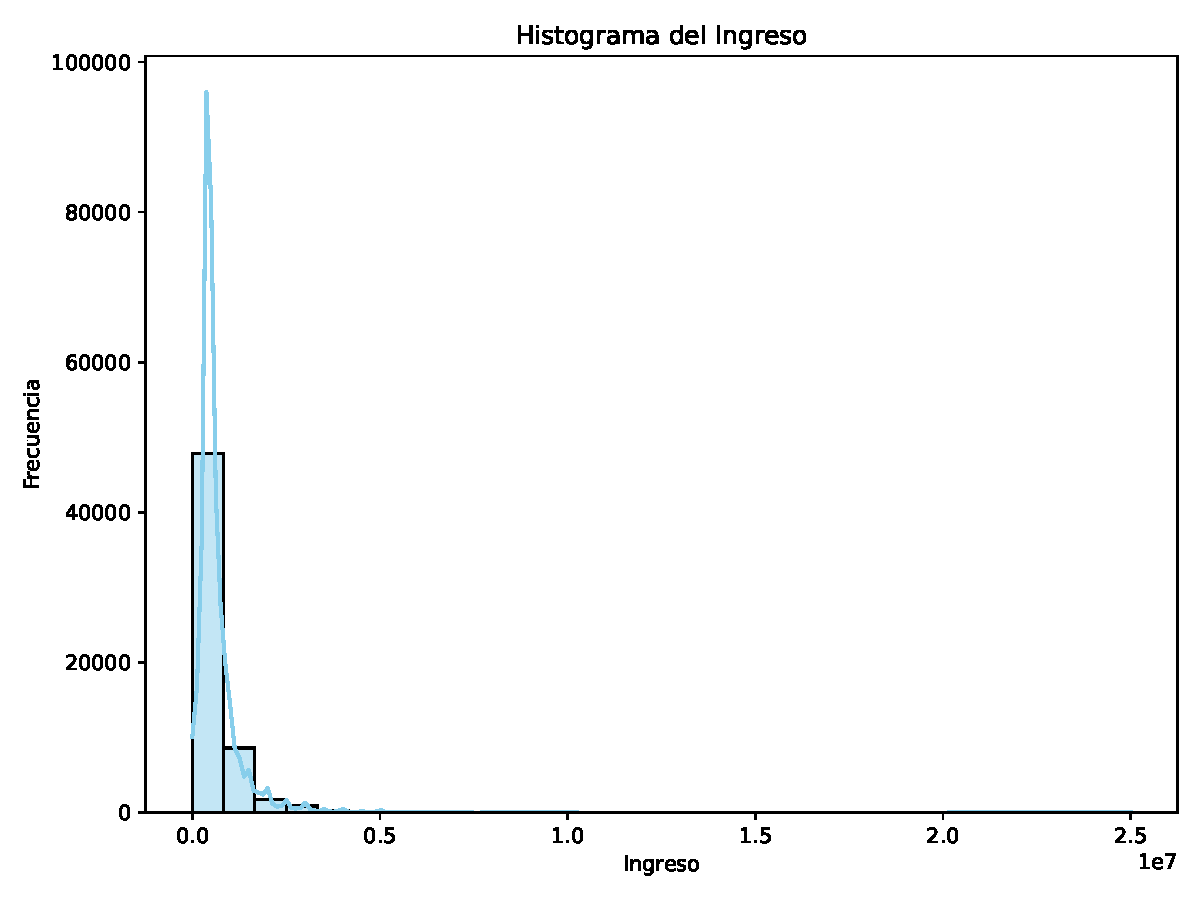
\includegraphics[width=1\textwidth]{../output/fig/HistoIngreso.pdf}
			\caption{\label{1a} Histograma Ingreso}
		\end{subfigure}
		\hfill
		\begin{subfigure}[b]{0.49\textwidth}
			\centering
			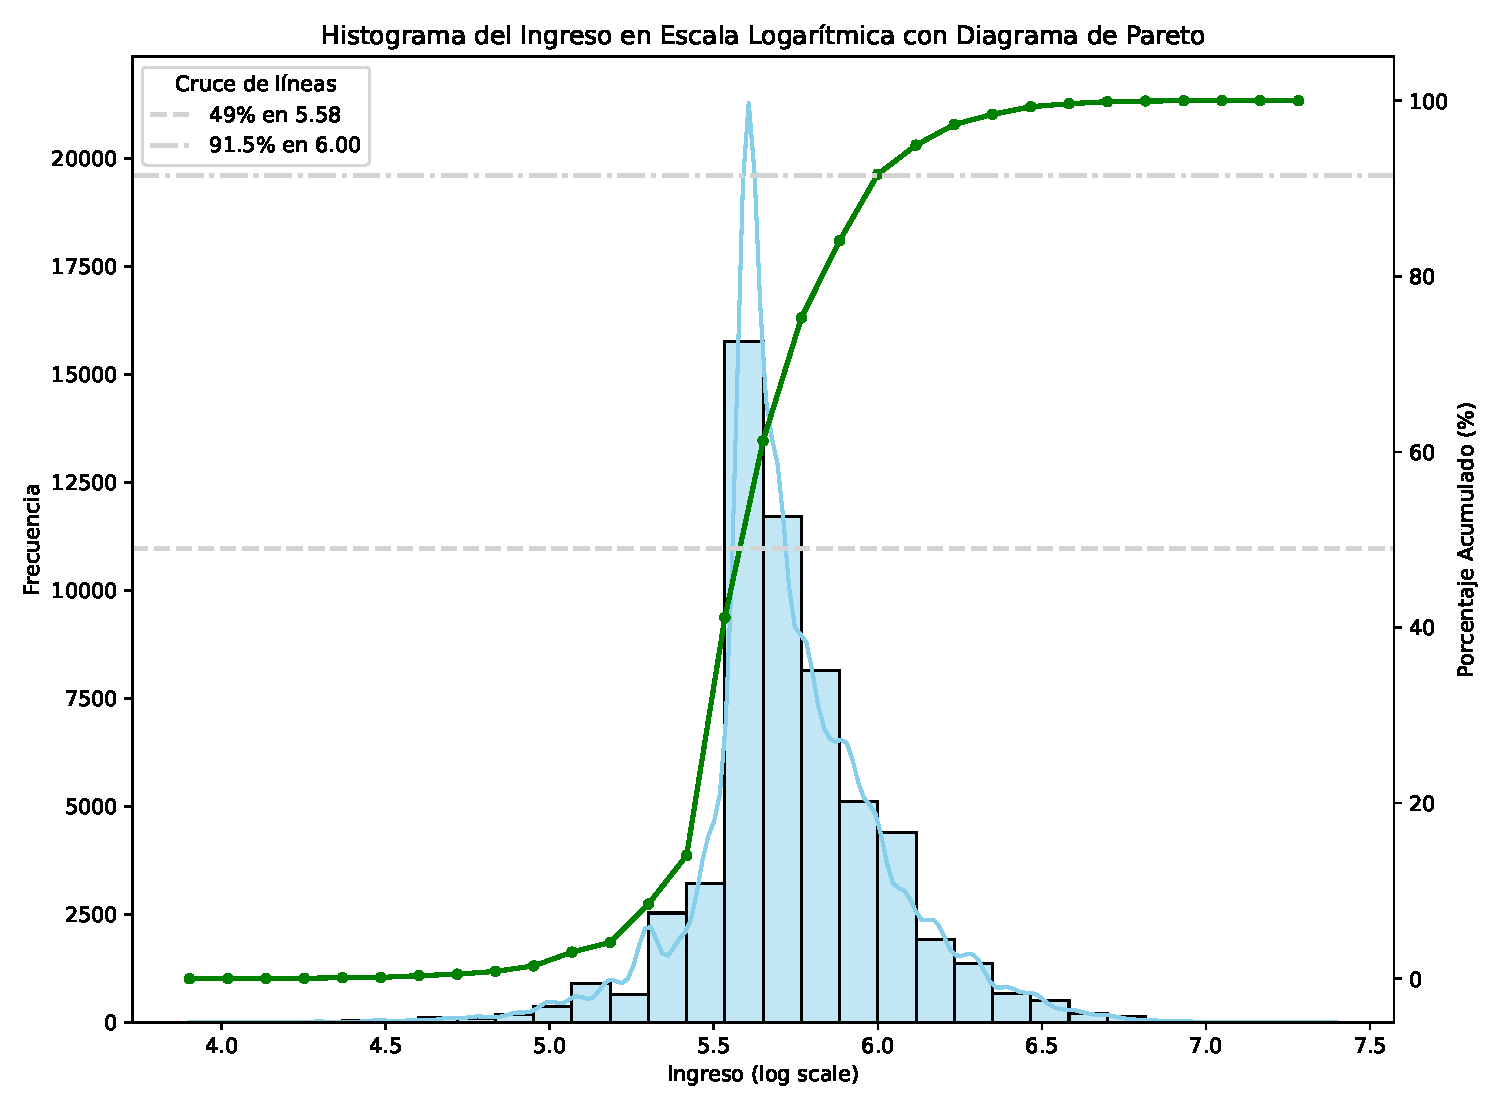
\includegraphics[width = 1\textwidth]{../output/fig/HistoIng_loglogPareto.pdf}
			\caption{\label{1b} fig.\ref{1a} en Escala Logarítmica + Diagrama de Pareto}
		\end{subfigure}
		\caption{Histogramas de Ingreso}
		\label{01fig}
	\end{figure}
	
	\begin{table}[htbp]
		\centering
		\begin{tabularx}{\textwidth}{|X|X|X|}
			\hline
			Fecha de Cambio & 18 a 65 años & Ley y Fecha de Promulgación\\
			\hline
			01-ene-2022 & 350.000 & 21.360 (05-07-2021) \\\hline
			01-may-2022 & 380.000 & 21.456 (26-05-2022) \\\hline
			01-ago-2022 & 400.000 & 21.456 (26-05-2022) \\\hline
		\end{tabularx}
		\caption{\label{tab} Sueldo mínimo 2022. (Fuente \cite{cyma})}
	\end{table}
		
	\FloatBarrier
	
	Como podemos apreciar en los gráficos de la Figura \ref{01fig}, existe una gran cantidad de personas con niveles de ingresos bajoa, mientras que los salarios más altos están concentrados en una minoría. Revisando a detalle el histograma de ingresos de la Figura \ref{1a}, se aprecia un primer “bin” (barra) enorme comparado a los demás. Considerando que el gráfico se encuentra en un rango de $0$ a $1\times10^{7}$ (0 a 10 millones), vemos que esa barra concentra los sueldos inferiores o iguales a \textdollar1.000.000.\\
	
	Para apreciar mejor la distribución de los sueldos, en la Figura \ref{1b} se realizó un histograma en escala logarítmica (\(\log_{10}\)) junto con un diagrama de Pareto, en el cual podemos apreciar que el cruce del 49\% se encuentra en $x=5.58$ (correspondiente a $10^{5.58}$ según la escala), lo que equivale a un sueldo de \textdollar380.189.\\
	
	Observando el Cuadro \ref{tab}, podemos apreciar que, entre mayo y agosto, el sueldo mínimo fue de \textdollar380.000. Tomándolo como referencia para el año y despreciando la diferencia de \textdollar189 de la gráfica, podemos decir que casi el 50\% de la población recibía el sueldo mínimo o menos, lo cual es una cifra bastante significativa. Además de eso, podemos observar que, siguiendo la misma lógica, el 91.5\% en $x=6$ implica que ese porcentaje de la población recibe sueldos iguales o inferiores a \textdollar1.000.000, siendo una cantidad muy importante de la población.
	
	\FloatBarrier
	
	\begin{figure}[htbp]
		\centering
		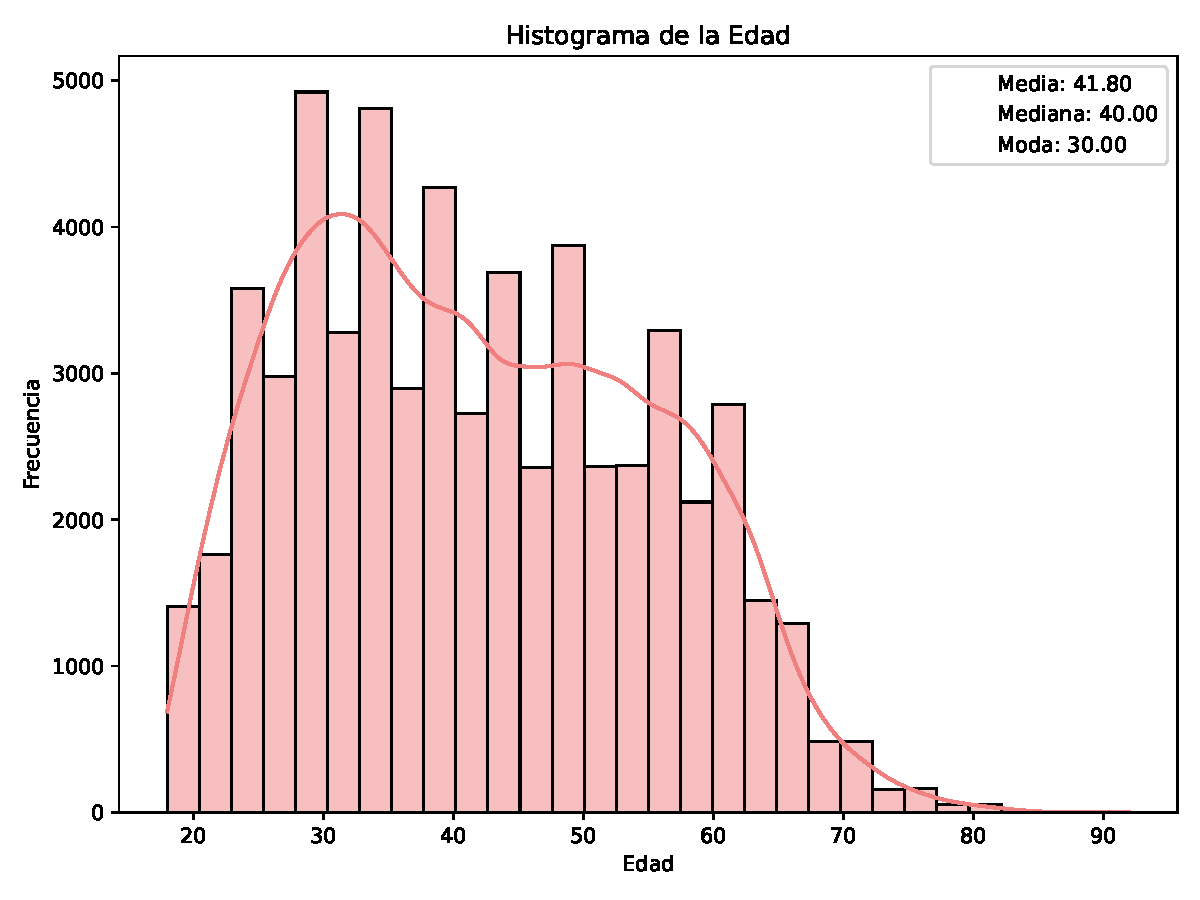
\includegraphics[width=0.65\textwidth]{../output/fig/HistoEdad.pdf}
		\caption{\label{02fig} Histograma Edad}
	\end{figure}
	
	\FloatBarrier
	
	En la Figura \ref{02fig}, apreciamos que la distribución de edades en la encuesta se asemeja bastante a una distribución normal, con sus MTC (Medidas de Tendencia Central), bastante cercanas al centro, con una media de $41.8$, mediana de $40$ y moda de $30$. Por lo tanto, en los gráficos que incluyen diferenciaciones según la edad, no deberíamos esperar inclinaciones pronunciadas hacia ningún lado.
	
	\FloatBarrier
	
	
	\begin{figure}[htbp]
		\centering
		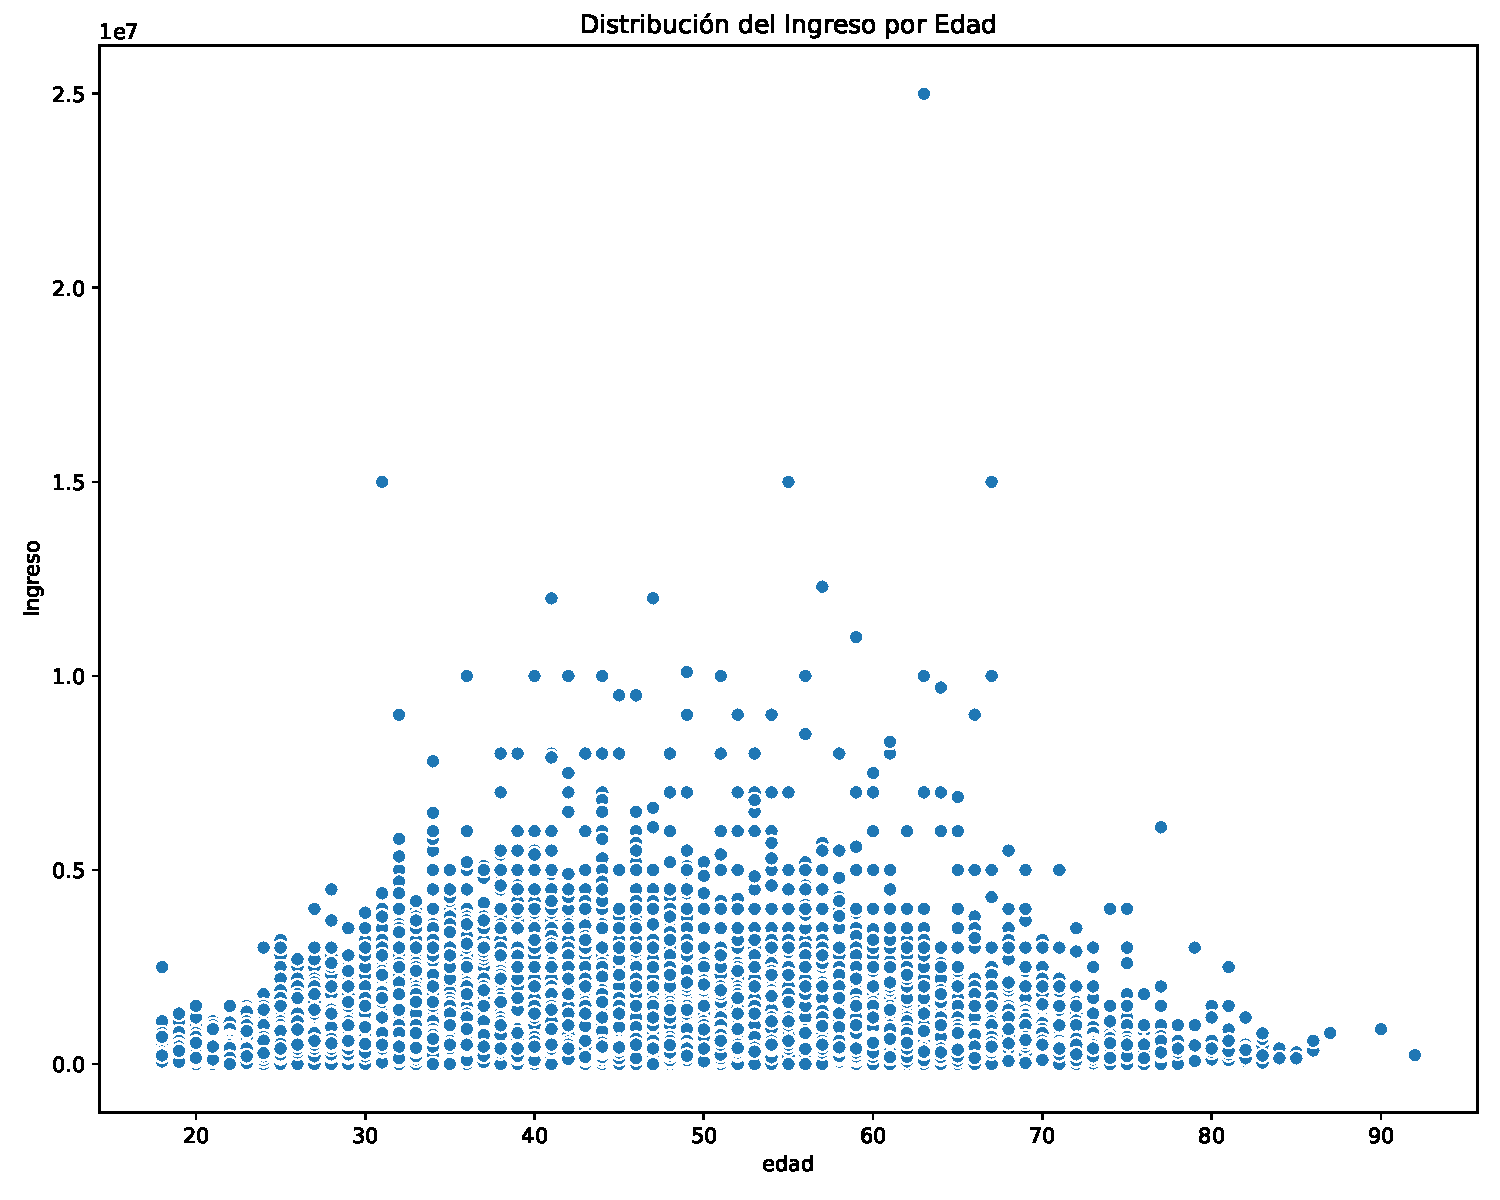
\includegraphics[width=0.65\textwidth]{../output/fig/DistIngEdad.pdf}
		\caption{\label{03fig} Distribución Ingresos Según Edad}
	\end{figure}
	
	\FloatBarrier
	
	Revisando la Figura \ref{03fig}, podemos observar que los ingresos más altos se concentran en las edades centrales, es decir, que la población más joven y la población más adulta (adultos mayores), son quienes reciben los menores ingresos.
	
	\FloatBarrier
	
	\begin{figure}[htbp]
		\centering
		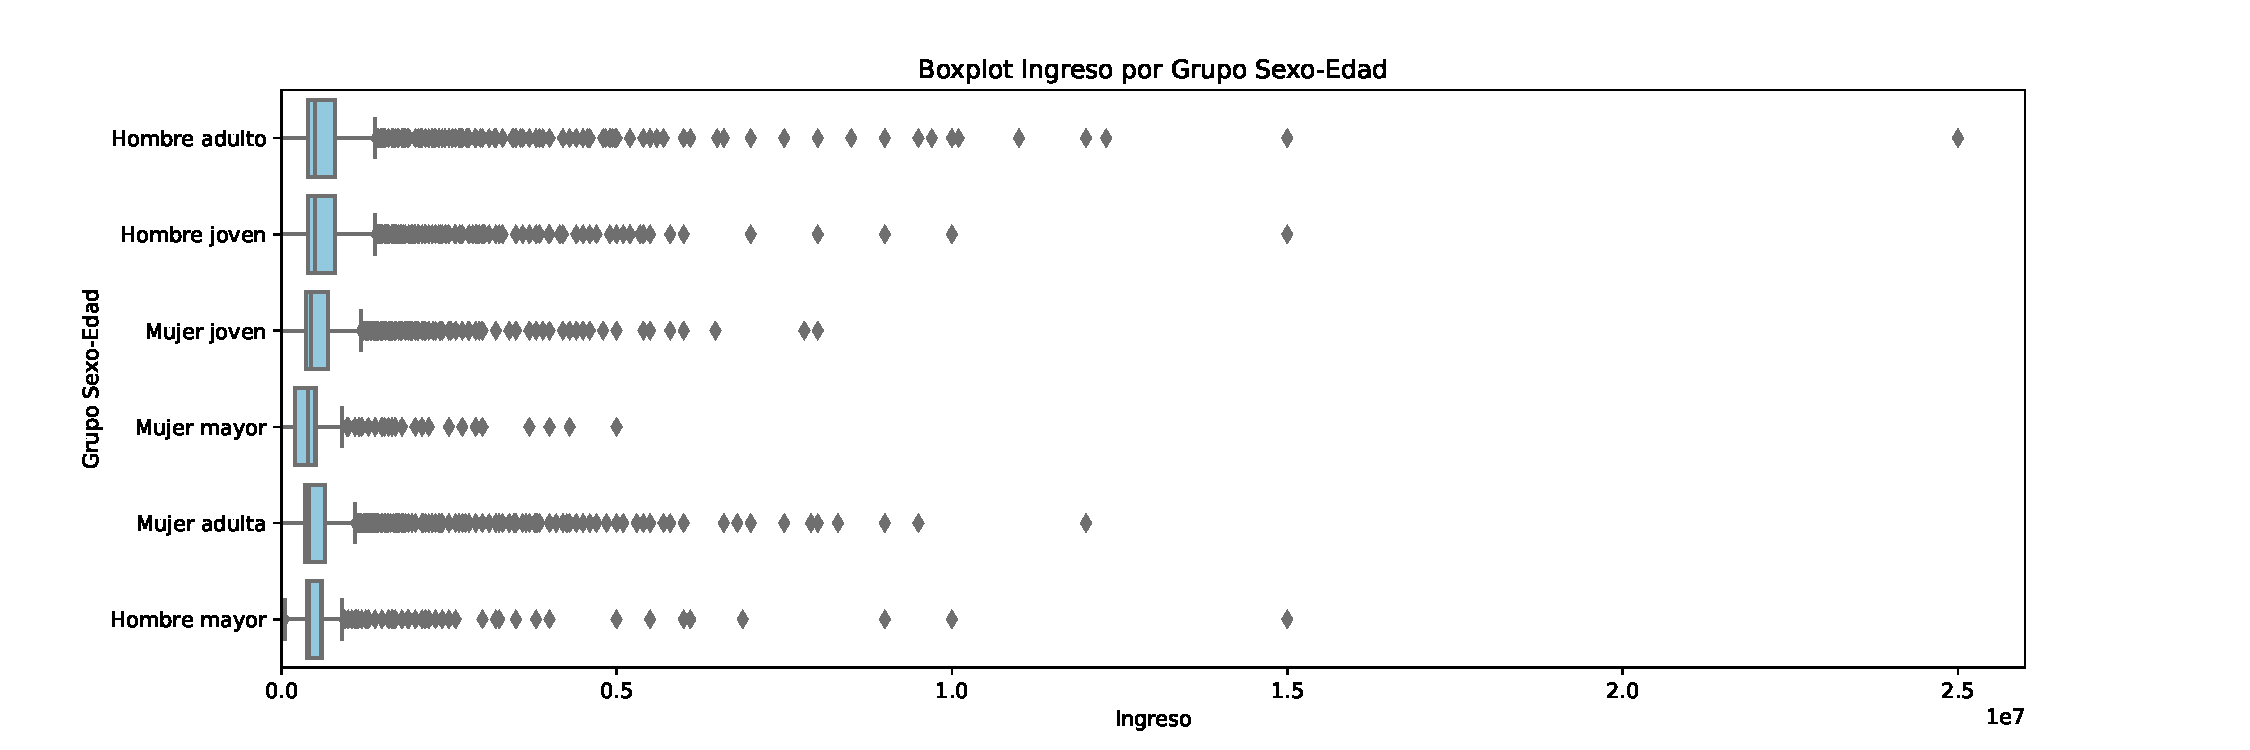
\includegraphics[width=0.65\textwidth]{../output/fig/BoxIngSexoEdad.pdf}
		\caption{\label{04fig} Boxplot Ingresos Según Sexo y Edad}
	\end{figure}
	
	\FloatBarrier
	
	En la Figura \ref{04fig} se observa una presencia significativa de valores atípicos que se alejan considerablemente de las medidas de tendencia central (MTC). Estos valores, especialmente los más extremos o alejados, provocan que las cajas del boxplot sean considerablemente más pequeñas, lo cual afecta la visualización y la interpretación de la distribución de ingresos según sexo y edad.
	
	\FloatBarrier
	
	\begin{figure}[htbp]
		\centering
		\begin{subfigure}[b]{0.49\textwidth}
			\centering
			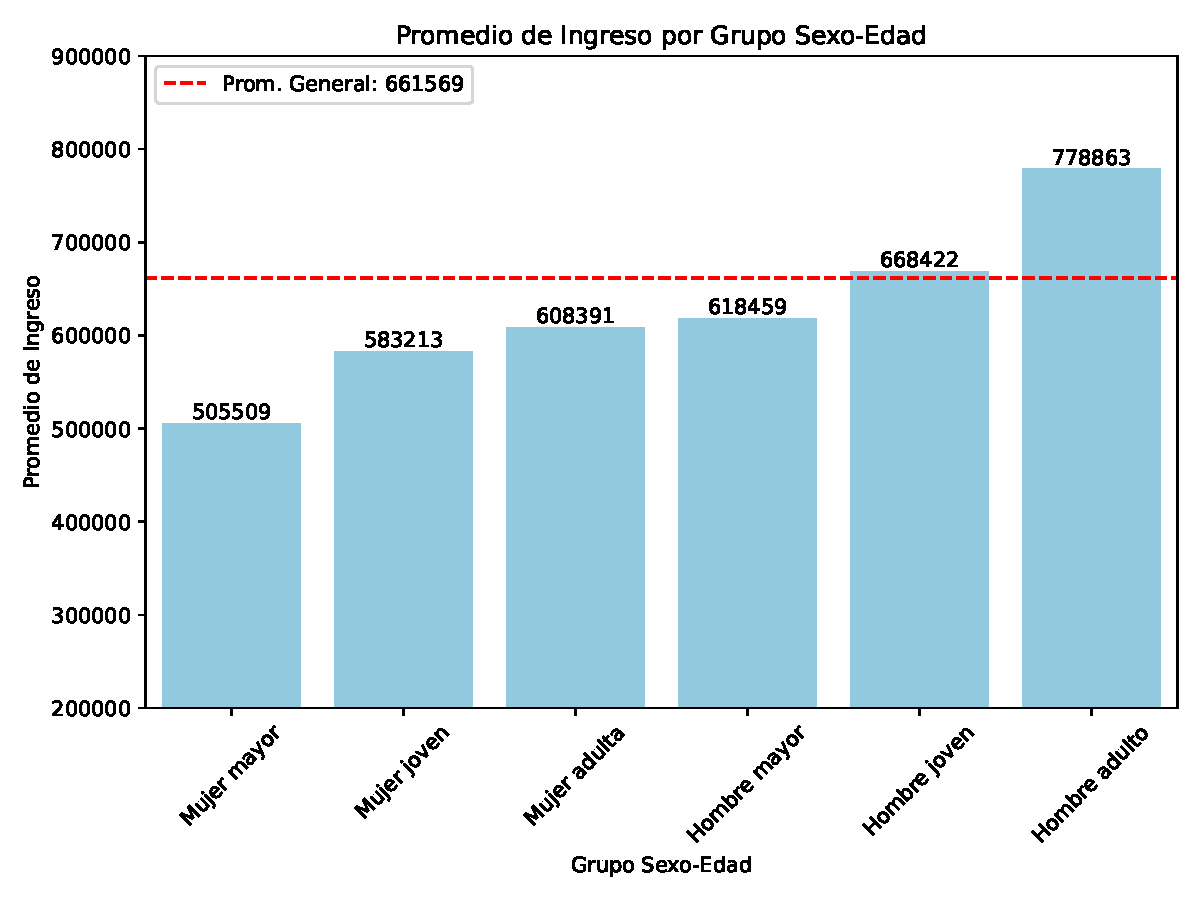
\includegraphics[width=1\textwidth]{../output/fig/PromIngSexoEdad.pdf}
			\caption{\label{5a} Sexo y Edad}
		\end{subfigure}
		\hfill
		\begin{subfigure}[b]{0.49\textwidth}
			\centering
			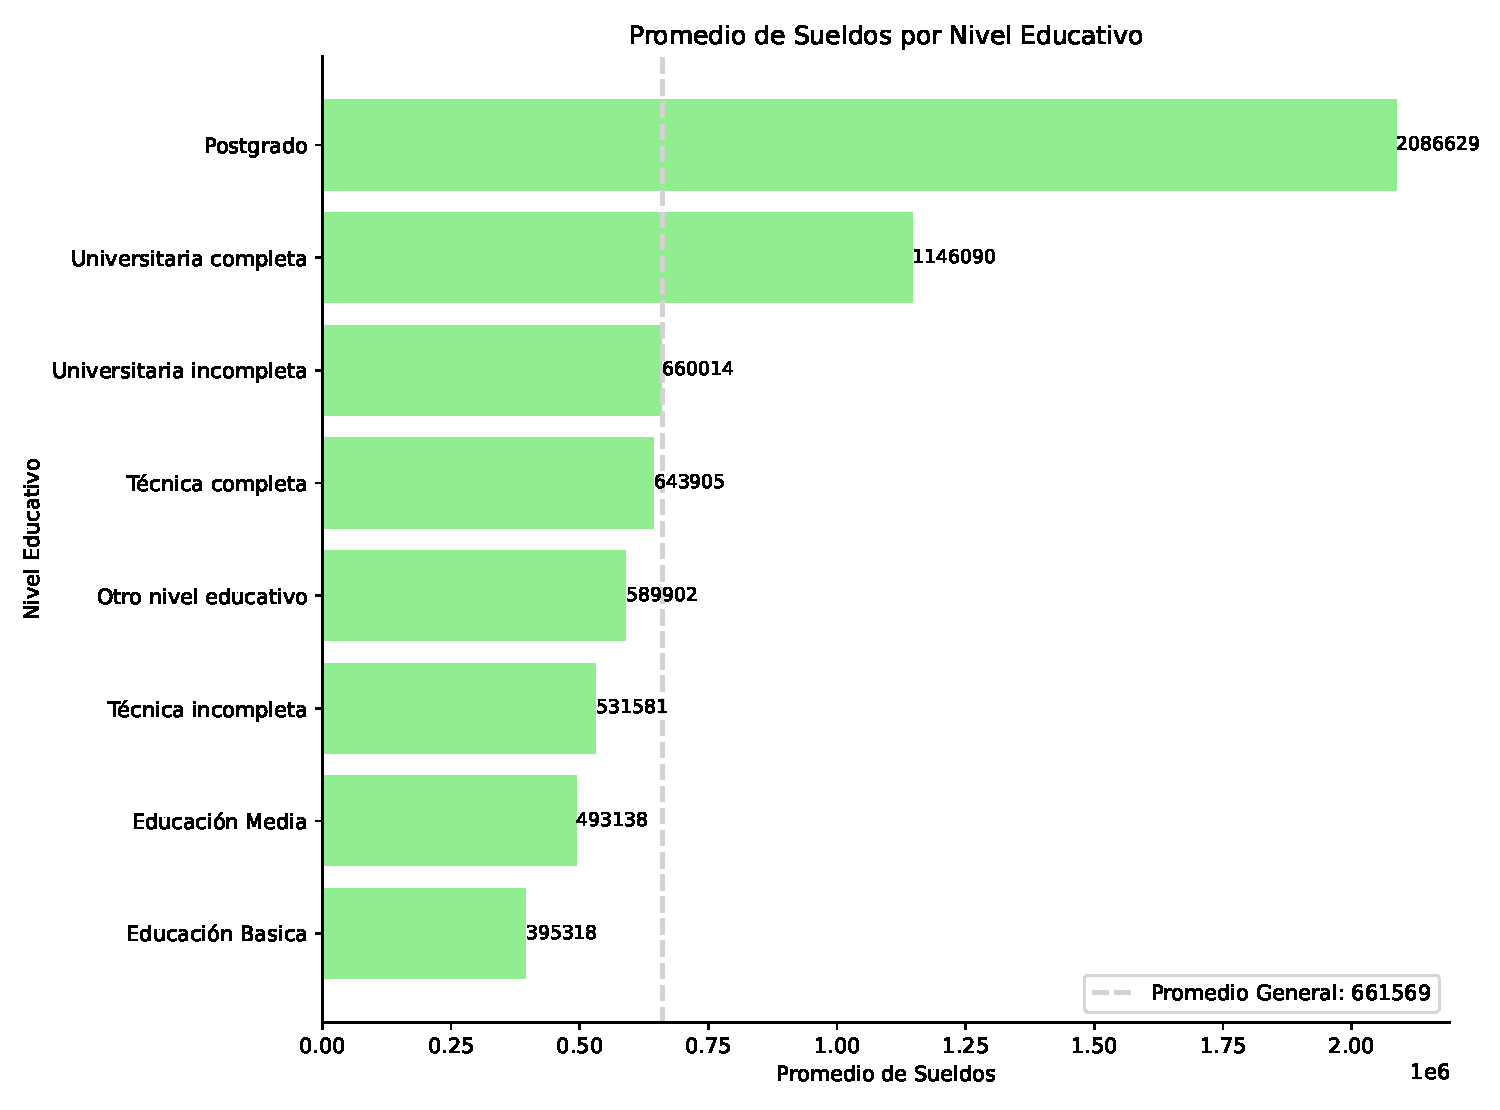
\includegraphics[width=1\textwidth]{../output/fig/PromIngEduca.pdf}
			\caption{\label{5b} Nivel Educacional}
		\end{subfigure}
		\caption{Promedio de Ingresos por Sexo, Edad y Nivel Educacional}
		\label{05fig}
	\end{figure}
	
	\FloatBarrier
	
	Respecto a la Figura \ref{05fig} se presentan dos gráficos significativos para el análisis del ingreso principal.\\
	
	Por un lado, en la Figura \ref{5a}, se muestran los promedios de ingresos según sexo y edad. Observamos que las mujeres en todos los grupos etarios tienen un promedio inferior al de los hombres. Vemos que, el promedio más alto para mujeres corresponde a las “Mujeres adultas” con \textdollar608.391, seguido por las “Mujeres jóvenes”, y finalmente las “Mujeres mayores” con el promedio más bajo en la gráfica. Por otro lado, los hombres muestran los tres promedios de ingresos principales más altos, siendo el más alto el correspondiente a los “Hombres adultos” con \textdollar778.863, seguido por los “Hombres jóvenes”, y finalmente los “Hombres mayores”.\\
	
	Estos datos coinciden con lo analizado en la Figura \ref{03fig}, donde se mencionaba que los adultos mayores y los jóvenes poseían menores ingresos. Sin embargo, aquí observamos que, en general, los adultos mayores tienen los ingresos más bajos, seguidos por los jóvenes y finalmente los adultos con los ingresos más altos. Además, notamos una diferencia significativa en los ingresos según el sexo, ya que las mujeres en todos los grupos etarios muestran ingresos inferiores incluso al menor ingreso observado en hombres. Como dato adicional, creo importante mencionar que los grupos de “Hombre joven” y “Hombre adulto”, son los únicos que están por encima de la media general de ingresos (\textdollar661.569).\\
	
	En el lado de la Figura \ref{5b}, apreciamos algo que era bastante esperable, a mayor nivel educativo, mayores son los ingresos. Observamos que el menor promedio de ingresos es de quienes cuentan solo con educación básica, mostrando un valor de \textdollar395.318. Mientras que, el mayor promedio de ingresos corresponde a las personas que estudiaron un postgrado, con una media de \textdollar2.086.629, seguido de quienes cuentan con carrera universitaria completa, que tienen un promedio de \textdollar1.146.090. Cabe destacar que estos dos grupos son los únicos que superan el promedio general de ingresos de \textdollar661.569.\\
	
	De igual manera, llama la atención que los ingresos de quienes pertenecen al grupo con educación universitaria incompleta estén sobre el promedio de quienes tienen educación técnica completa, con ingresos promedio de \textdollar660.014 (muy cercano a la media) frente a los \textdollar643.905 respectivamente.\\
	
	\FloatBarrier
	
	\begin{figure}[htbp]
		\centering
		\begin{subfigure}[b]{0.49\textwidth}
			\centering
			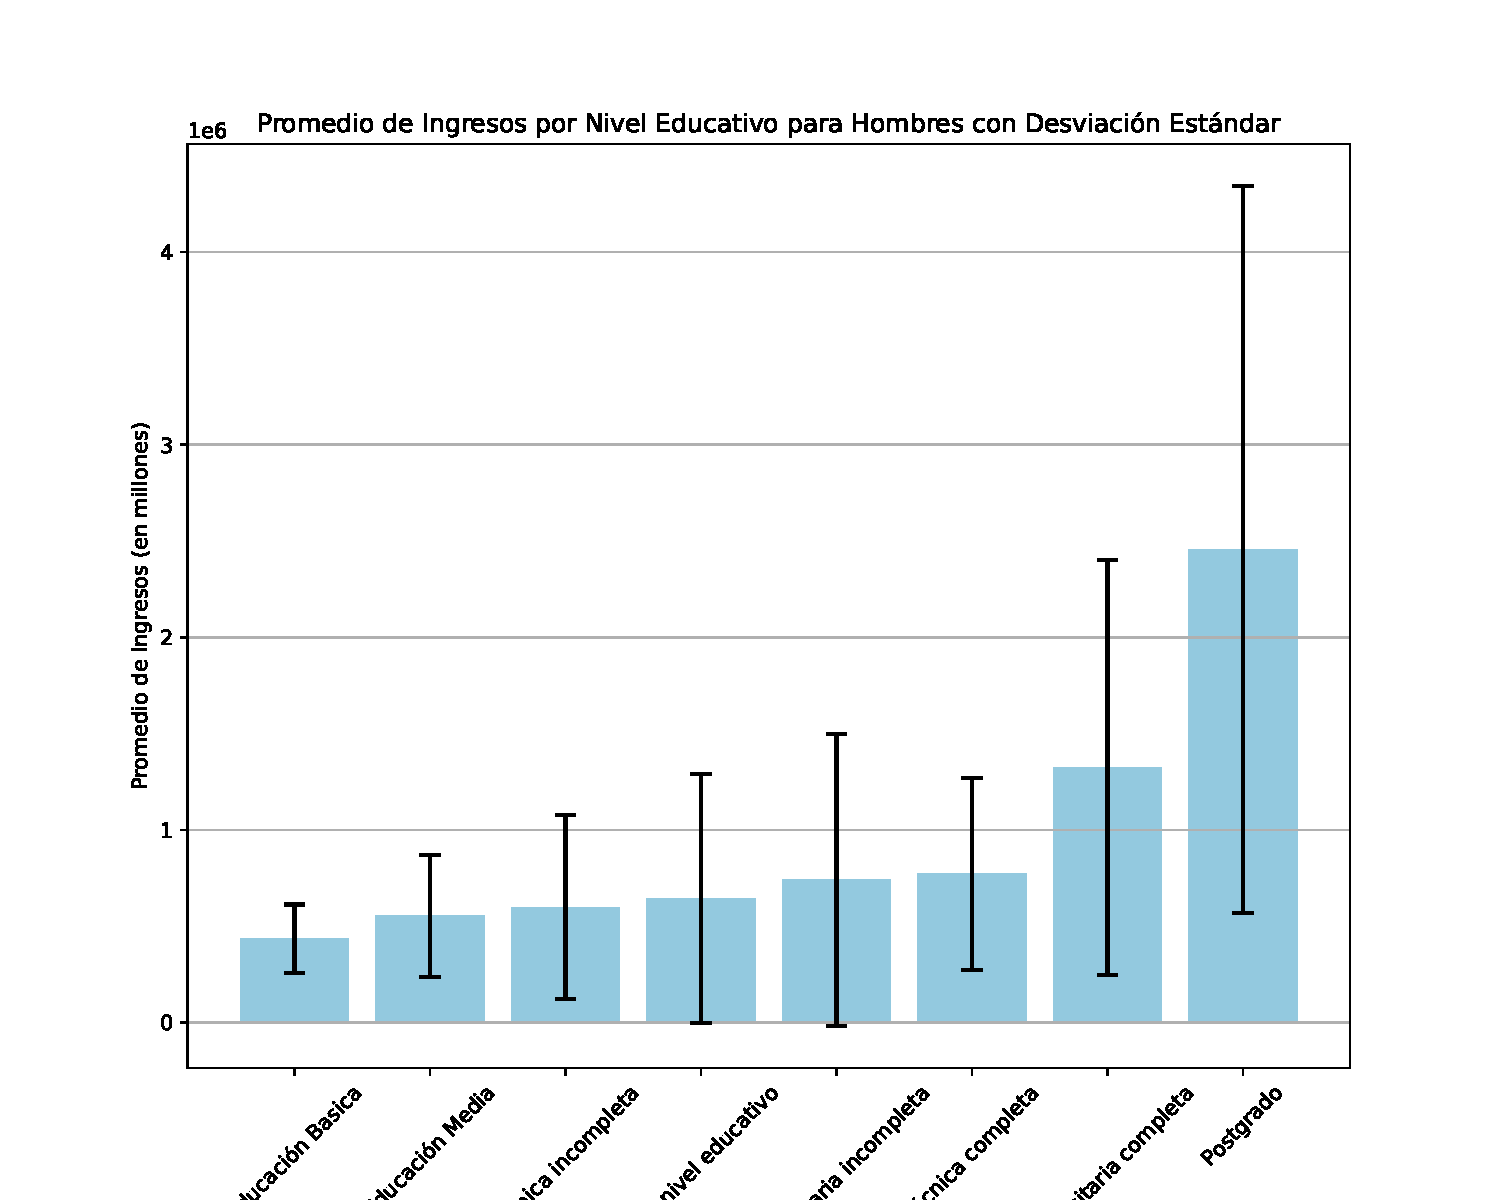
\includegraphics[width=1\textwidth]{../output/fig/PromIngH_EducaDE.pdf}
			\caption{\label{6a} Hombres}
		\end{subfigure}
		\hfill
		\begin{subfigure}[b]{0.49\textwidth}
			\centering
			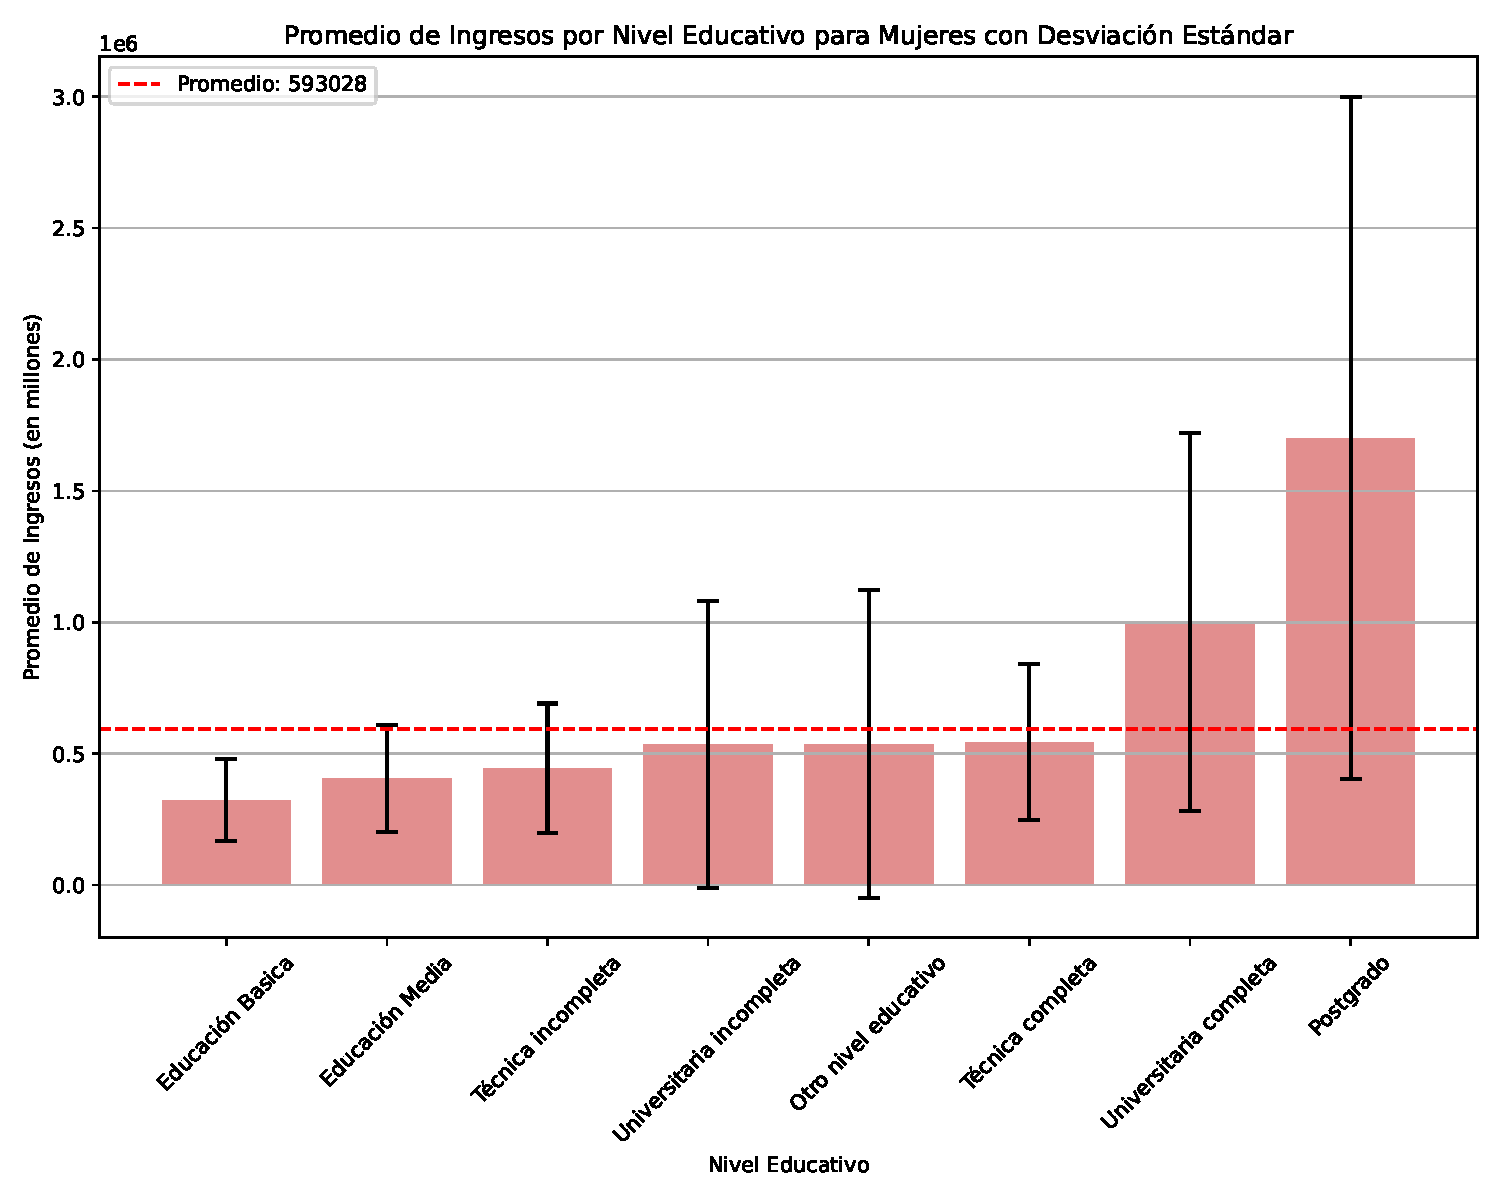
\includegraphics[width=1\textwidth]{../output/fig/PromIngM_EducaDE.pdf}
			\caption{\label{6b} Mujeres}
		\end{subfigure}
		\caption{Promedio de Ingresos por Nivel Educacional y Desviación Estándar para Hombres y Mujeres}
		\label{06fig}
	\end{figure}
	
	\FloatBarrier
	
	De los gráficos de la Figura \ref{06fig} podemos ver que nuevamente el nivel educacional es una variable muy importante en cuanto al tamaño del ingreso, al igual que en la Figura \ref{5b} a mayor nivel educacional, mayor es el ingreso. Apreciamos que lo anterior es aplicable para hombres y mujeres.\\
	
	Sin embargo, vemos una diferencia importante en cuanto al promedio general de ingresos de hombres y mujeres, podemos observar en la Figura \ref{6a} que la media de ingresos en hombres es de \textdollar717.972, la cual es superada por los hombres con educación universitaria incompleta, técnica completa, universitaria completa y postgrado. Mientras que en la Figura \ref{6b} vemos que la media de ingresos es de \textdollar593.028, representando una diferencia de \textdollar124.944 respecto a los hombres, un 17.4\% inferior respectivamente, lo cual es bastante en términos de equidad salarial y disparidades económicas de género. La media de mujeres, por otra parte, sólo la superan aquellas que cuentan con educación universitaria completa y postgrado.\\
	
	En ambos gráficos, las barras de desviación estándar representan la variabilidad o dispersión de los ingresos en cada nivel educativo (a barras más altas o grandes, mayor es la dispersión del ingreso). En la Figura \ref{6a} (hombres), las barras que indican mayor desviación, corresponden a los niveles educativos de universitaria incompleta, completa y postgrado. Mientras que, en la Figura \ref{6b} (mujeres), notamos que las barras indican una mayor desviación en aquellas mujeres con educación universitaria completa y postgrado.\\
	
	Por el contrario, las barras más pequeñas o estables podemos visualizarlas en quienes cuentan con educación básica y/o media, tanto en hombres como en mujeres.
		
	\FloatBarrier
	
	\begin{figure}[htbp]
		\centering
		\begin{subfigure}[b]{0.49\textwidth}
			\centering
			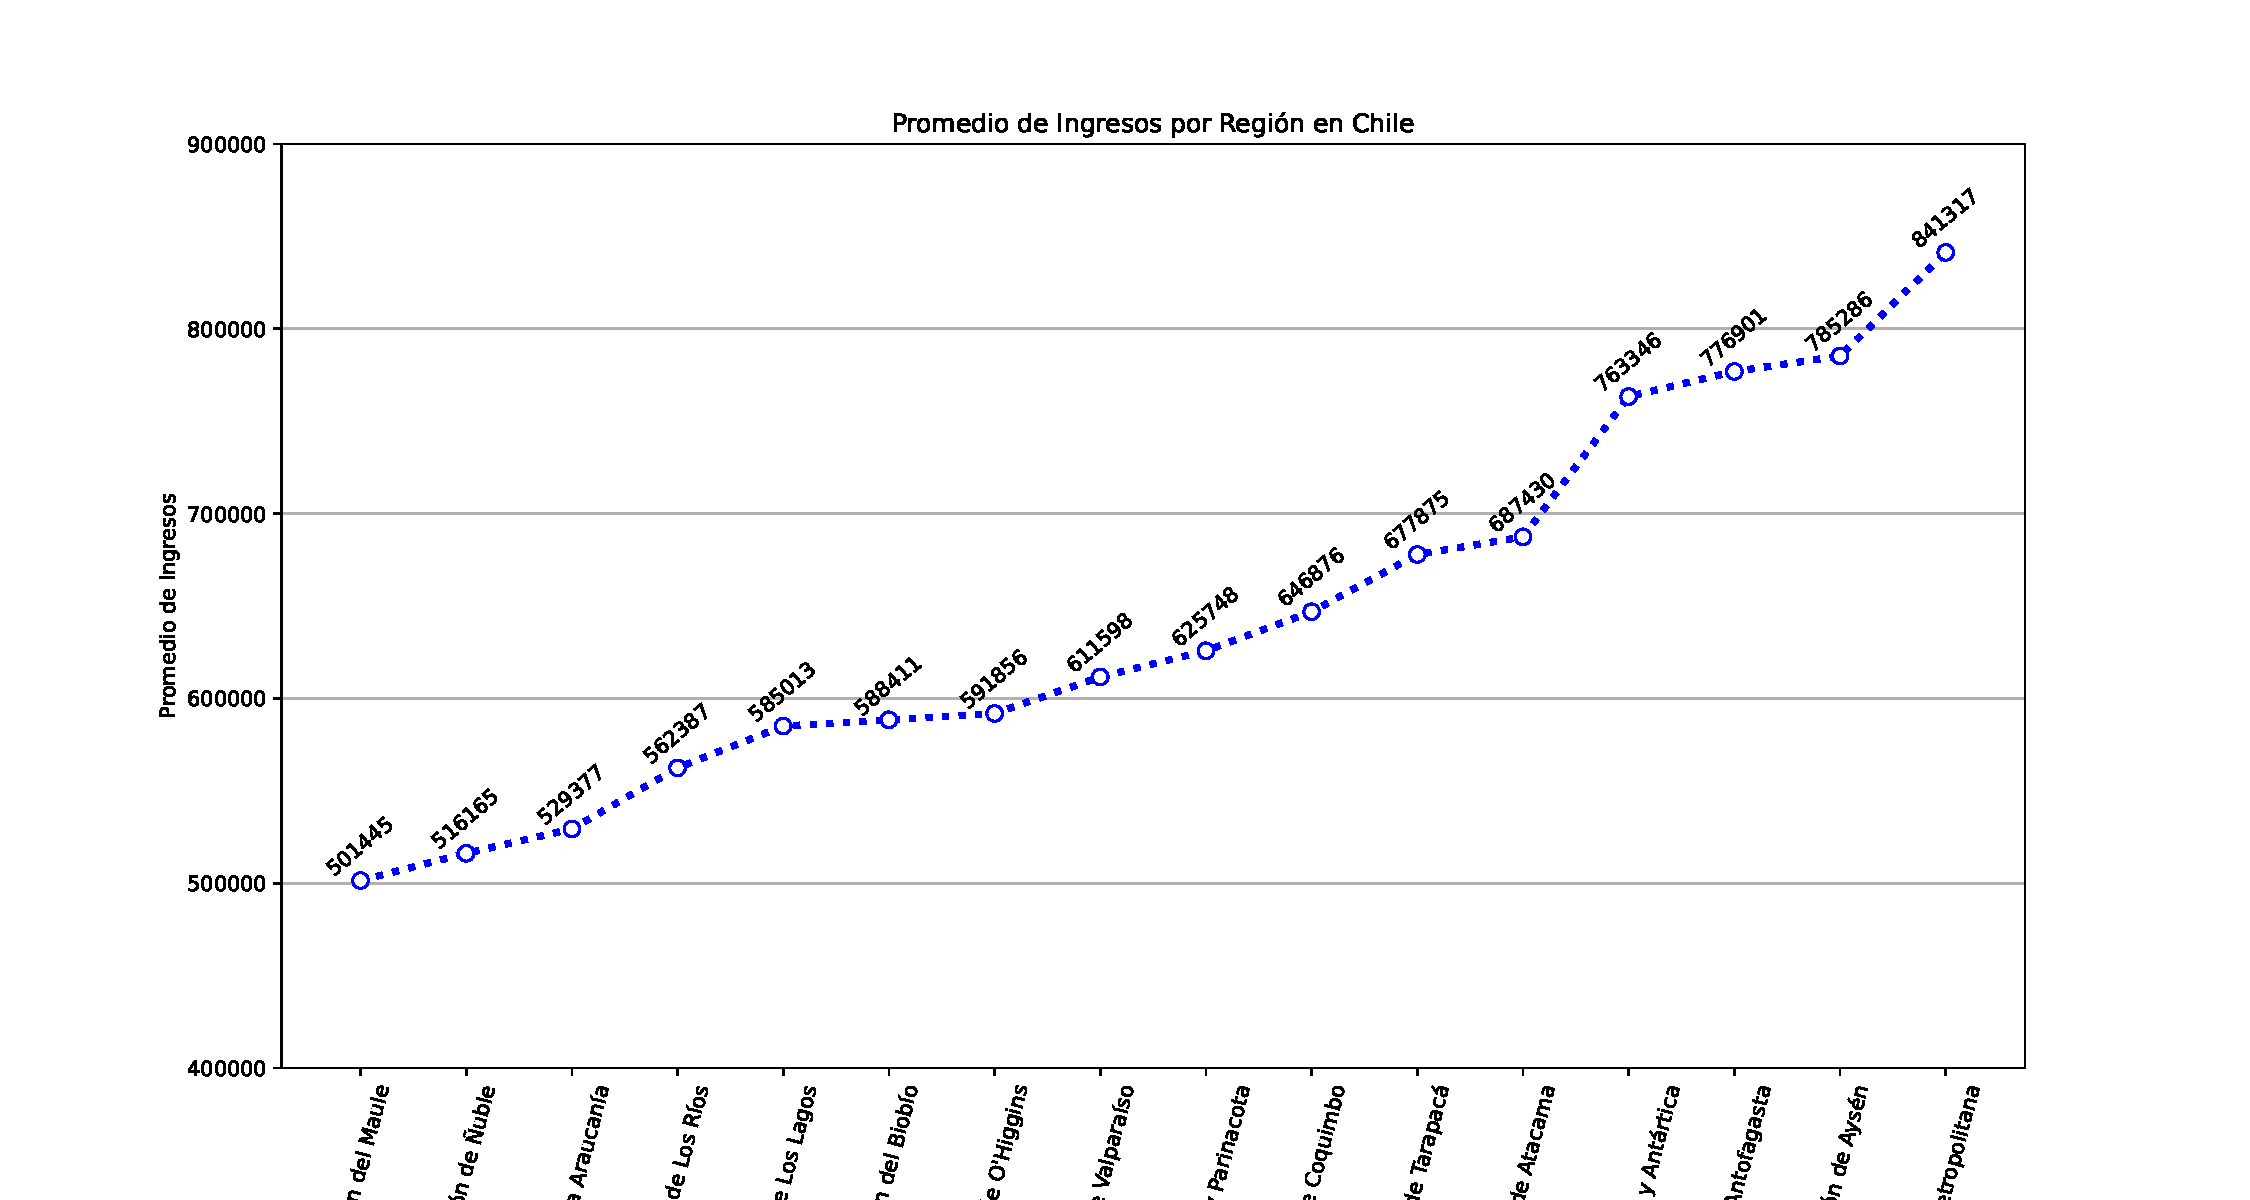
\includegraphics[width=1\textwidth]{../output/fig/PromIngRegion.pdf}
			\caption{\label{7a} Región}
		\end{subfigure}
		\hfill
		\begin{subfigure}[b]{0.49\textwidth}
			\centering
			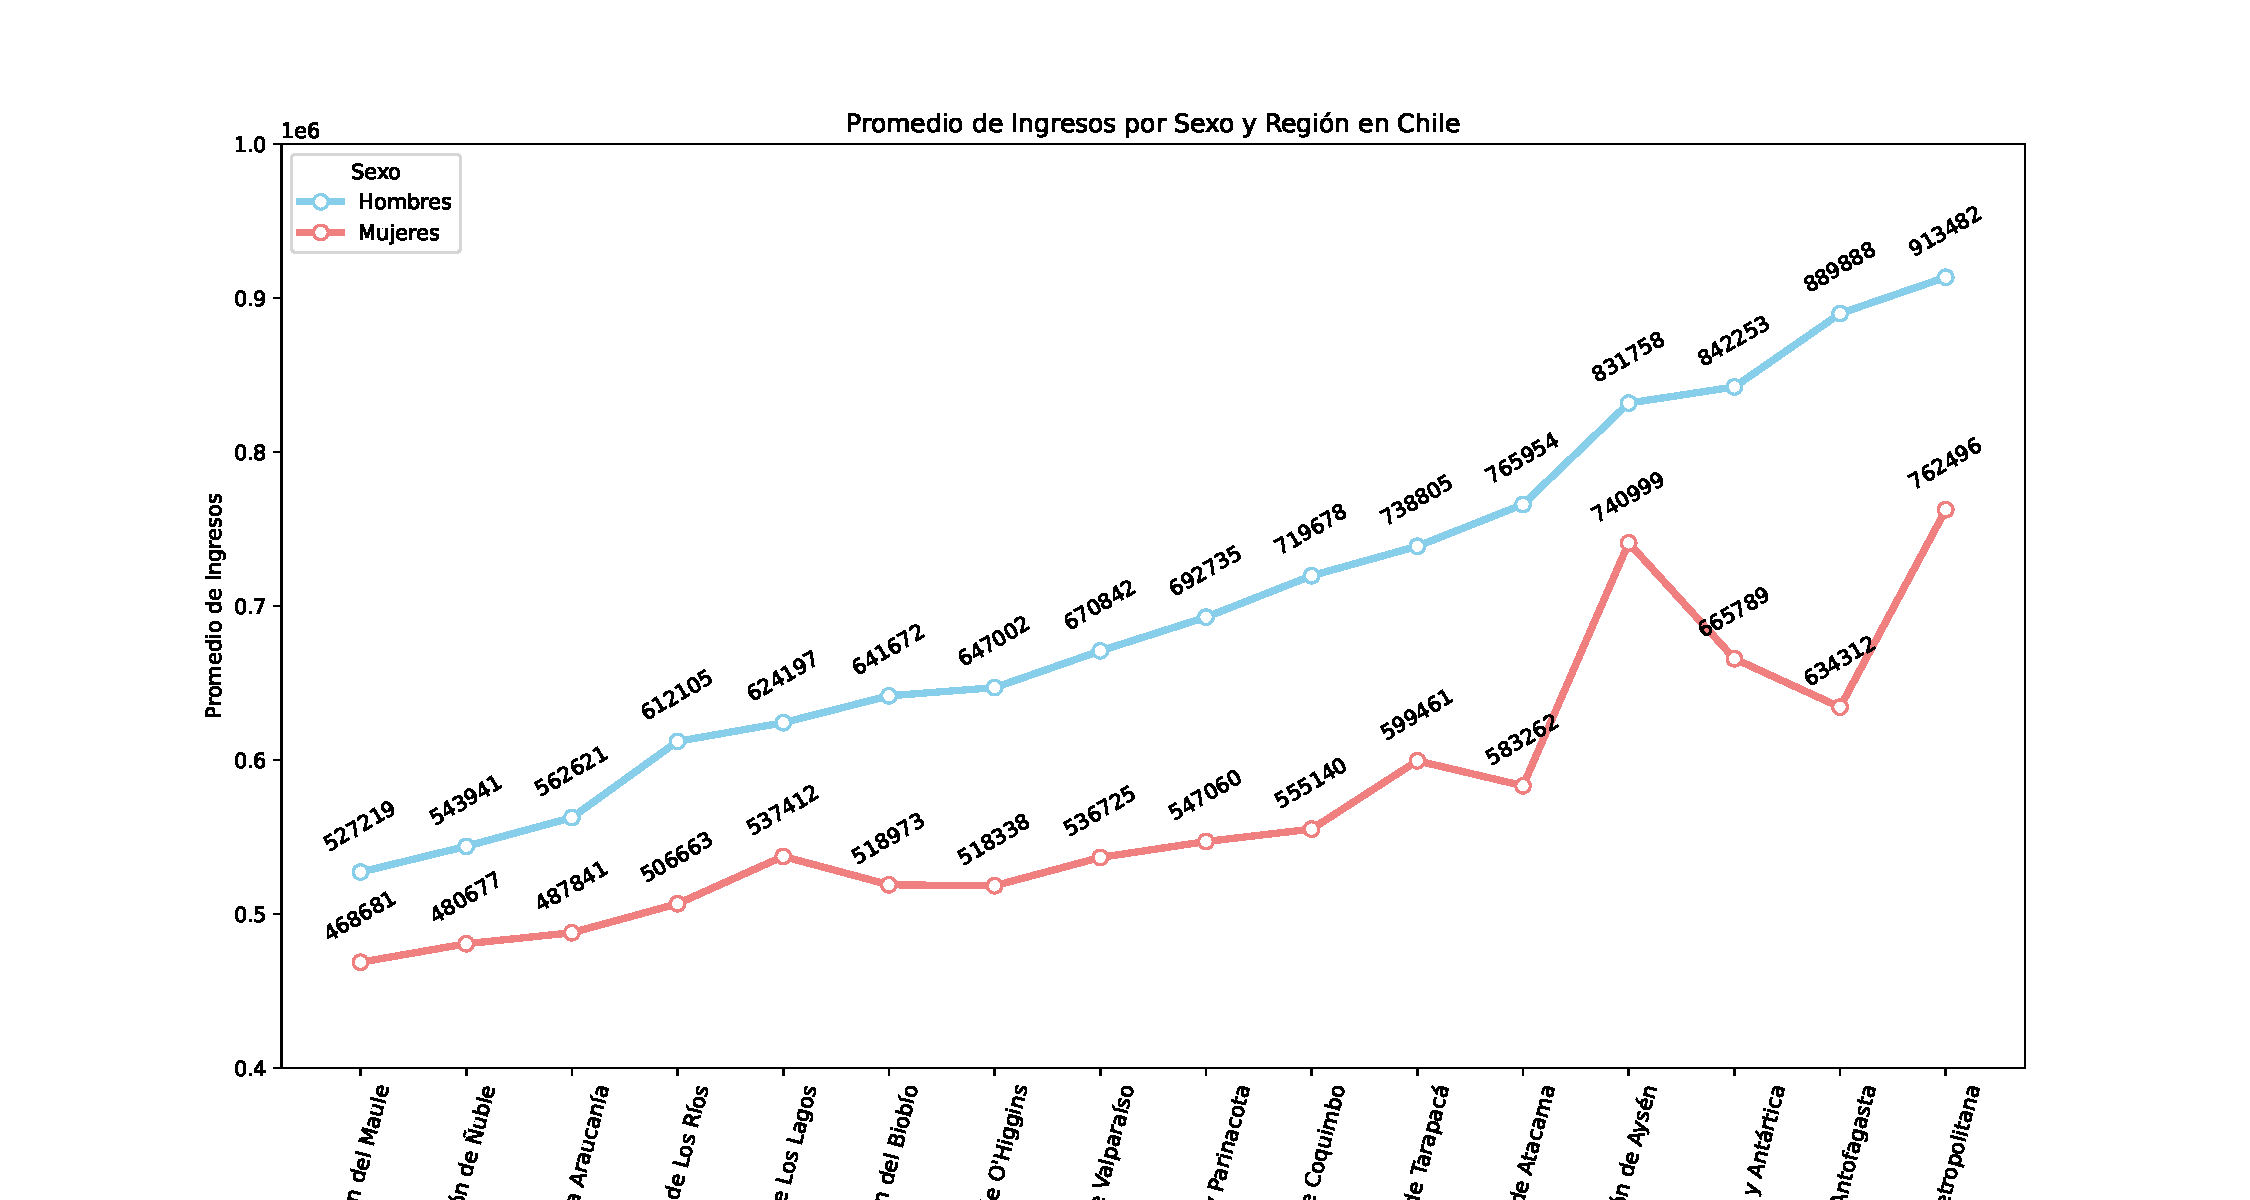
\includegraphics[width=1\textwidth]{../output/fig/PromIngSexoRegion.pdf}
			\caption{\label{7b} Sexo y Región}
		\end{subfigure}
		\caption{Promedio de Ingresos por Región y por Sexo y Región}
		\label{07fig}
	\end{figure}
	
	\FloatBarrier
	
	La Figura \ref{07fig}, nos muestra dos comparativas a nivel regional. Por un lado, en la Figura \ref{7a}, observamos que la Región Metropolitana cuenta con la media de ingresos más alta (\textdollar841.317), seguida de las regiones de Aysén, Antofagasta y Magallanes y Antártica. Ahora, revisando desde abajo, nos encontramos que la Región del Maule tiene los menores ingresos, con un promedio de \textdollar501.445, seguida las regiones de Ñuble, Araucanía y Los Ríos. En la misma gráfica, evidenciamos que 6 de las 16 regiones del país, superan la media general de ingresos (\textdollar661.569), estas son:
	
	\subsubsection*{Regiones que superan el promedio (de mayor a menor):}
	
	\begin{itemize}
		\item Región Metropolitana
		\item Región de Aysén
		\item Región de Antofagasta
		\item Región de Magallanes y Antártica
		\item Región de Atacama
		\item Región de Tarapacá
	\end{itemize}
	
	Detallando ahora en la Figura \ref{7b}, podemos constatar lo que hemos visto en cada gráfica anterior que incluya la variable de sexo, en cada una de las regiones los hombres tienen un promedio de ingresos mayor al de las mujeres, según las líneas horizontales, incluso tienen una media salarial mayor al promedio general de ingresos, estando el sexo femenino, por debajo de ambos promedios en cuanto al ingreso. Las 4 regiones con mayores y menores ingresos para ambos sexos son las mismas que representa la Figura \ref{7a}.\\
	
	Sin embargo, en el caso de los hombres se evidencia que 9 de las 16 regiones sobrepasa el promedio general de ingresos, 7 de las 16 regiones sobrepasan el promedio de ingresos de los mismos hombres y en 13 de las 16 regiones sobrepasan el promedio de ingresos de las mujeres.\\
	
	Por contraparte, constatamos que las mujeres sobrepasan el promedio general de ingresos en solo 3 de las 16 regiones del país, mientras que en 5 de las 16 regiones sobrepasan su propia media de ingresos y solamente en 2 de las 16 regiones sobrepasan el promedio de ingresos de los hombres.\\
	
	Considero preocupantes las cifras anteriormente mencionadas, ya que indican que el hombre puede obtener mejores oportunidades laborales en la mayor parte del país.\\
	
	Por último, podríamos decir que las mejores regiones en cuanto a sueldos para ambos sexos, serían la Region Metropolitana, seguida de la Región de Aysén, ya que presentan los ingresos más altos en general de toda la Figura \ref{07fig}.
	
	\FloatBarrier
	
	\section*{Conclusión}
	
	Finalizando este informe, nos encontramos con varios puntos relevantes en cuanto al análisis del ingreso principal. Por una parte, en cuanto a la distribución de ingresos, notamos una clara concentración de ingresos más altos en las edades centrales, mientras que jóvenes y adultos mayores tienden a tener ingresos más bajos. Dentro de los descubrimientos más importantes, observamos que el 49\% de la población gozaba de un sueldo igual o inferior al mínimo, mientras que el 91.5\% obtenía ingresos menores a \textdollar1.000.000.\\
	
	En cuanto a las diferencias por género y equidad salarial, evidenciamos que los hombres tienen ingresos superiores a las mujeres en todos los grupos etarios, niveles educacionales analizados (especialmente los niveles más altos) e incluso en todas las regiones del país. Se presenta una significativa disparidad salarial y sugiere una brecha basada en el género.\\
	
	Por parte del nivel educativo, constatamos que a mayor nivel educativo, mayores son los ingresos promedio tanto para hombres, como para mujeres. Destacan en los resultados los grupos con educación universitaria completa y postgrado por tener ingresos considerablemente más altos y superiores al promedio general de ingresos en Chile. Sin embargo, como bien vimos, los niveles educativos más altos tienden a tener una mayor dispersión de ingresos, indicando una gran variabilidad en los diferentes salarios.\\
	
	\newpage
	\begin{thebibliography}{99}
		
		\bibitem{cyma}
		Sueldo Mínimo en Chile.
		CYMA Suite.
		\url{https://cymasuite.com/sueldo-minimo-chile}
		[Consulta: 21 de junio de 2024].
		
		\bibitem{casen2022}
		Observatorio Social - Ministerio de Desarrollo Social y Familia.
		\url{https://observatorio.ministeriodesarrollosocial.gob.cl/encuesta-casen-2022}
		[Consulta: 21 de junio de 2024].
		
	\end{thebibliography}
		
\end{document}